\documentclass[11pt,a4paper]{article}

\usepackage[T1]{fontenc}
\usepackage[utf8]{inputenc}
\usepackage[english]{babel}
\usepackage{lmodern}
\usepackage[
  a4paper,
  left=1.9cm,
  right=1.9cm,
  top=2.35cm,
  bottom=2.35cm,
  headheight=15pt
]{geometry}
\usepackage{microtype}
\usepackage{setspace}
\usepackage{amsmath,amssymb,mathtools}
\usepackage{graphicx}
\usepackage{float}
\usepackage{booktabs}
\usepackage{tabularx}
\usepackage{array}
\usepackage{siunitx}
\usepackage{caption}
\usepackage{enumitem}
\usepackage{xcolor}
\usepackage{xurl}
\usepackage{fancyhdr}
\usepackage{titlesec}
\usepackage[numbers,sort&compress]{natbib}
\usepackage{tikz}
\usetikzlibrary{arrows.meta,positioning}
\usepackage[hidelinks]{hyperref}
\usepackage[nameinlink,capitalise,noabbrev]{cleveref}

\definecolor{ReportBlue}{HTML}{1D4ED8}
\definecolor{ReportInk}{HTML}{1F2937}
\definecolor{ReportGrey}{HTML}{6B7280}
\definecolor{ReportLight}{HTML}{EFF6FF}

\hypersetup{
  pdftitle={Taxi Destination Prediction from Partial Trajectories},
  pdfsubject={ELEN0062 Project 3 technical report},
  pdfkeywords={taxi destination, machine learning, Haversine, ensemble, reproducibility},
  colorlinks=true,
  linkcolor=ReportBlue,
  citecolor=ReportBlue,
  urlcolor=ReportBlue
}

\graphicspath{{figures/}}
\setstretch{1.06}
\setlength{\parindent}{0pt}
\setlength{\parskip}{0.55em}
\setlist{nosep,leftmargin=1.6em}
\setcounter{secnumdepth}{3}

\titleformat{\section}
  {\Large\bfseries\color{ReportInk}}
  {\thesection}{0.7em}{}
\titleformat{\subsection}
  {\large\bfseries\color{ReportInk}}
  {\thesubsection}{0.65em}{}
\titleformat{\subsubsection}
  {\normalsize\bfseries\color{ReportInk}}
  {\thesubsubsection}{0.55em}{}

\pagestyle{fancy}
\fancyhf{}
\fancyhead[L]{\small Taxi Destination Prediction}
\fancyhead[R]{\small\nouppercase{\leftmark}}
\fancyfoot[C]{\thepage}
\renewcommand{\headrulewidth}{0.4pt}

\captionsetup{
  position=bottom,
  font=small,
  labelfont=bf,
  textfont=it,
  justification=justified,
  singlelinecheck=false
}

\sisetup{
  group-separator={,},
  group-minimum-digits=4,
  detect-all
}

\tikzset{
  workflow/.style={
    draw=ReportBlue,
    rounded corners=2pt,
    fill=ReportLight,
    align=center,
    minimum height=0.9cm,
    text width=2.55cm,
    font=\small
  },
  flowarrow/.style={-{Latex[length=2.2mm]},thick,draw=ReportGrey}
}


\begin{document}

\hypersetup{pageanchor=false}

\begin{titlepage}
  \centering
  \vspace*{1.2cm}
  {\Large ELEN0062 -- Introduction to Machine Learning\par}
  \vspace{0.55cm}
  {\color{ReportBlue}\rule{0.88\textwidth}{1.2pt}\par}
  \vspace{0.6cm}
  {\Huge\bfseries Taxi Destination Prediction\par}
  \vspace{0.35cm}
  {\LARGE From Partial Trajectories to a Reproducible Ensemble\par}
  \vspace{0.6cm}
  {\color{ReportBlue}\rule{0.88\textwidth}{1.2pt}\par}
  \vspace{0.75cm}
  {\Large Project 3 -- Competition\par}
  \vspace{0.3cm}
  {\large Technical report\par}
  \vspace{0.45cm}
  {\Large\bfseries Louis Hogge\par}
  \vspace{0.75cm}
  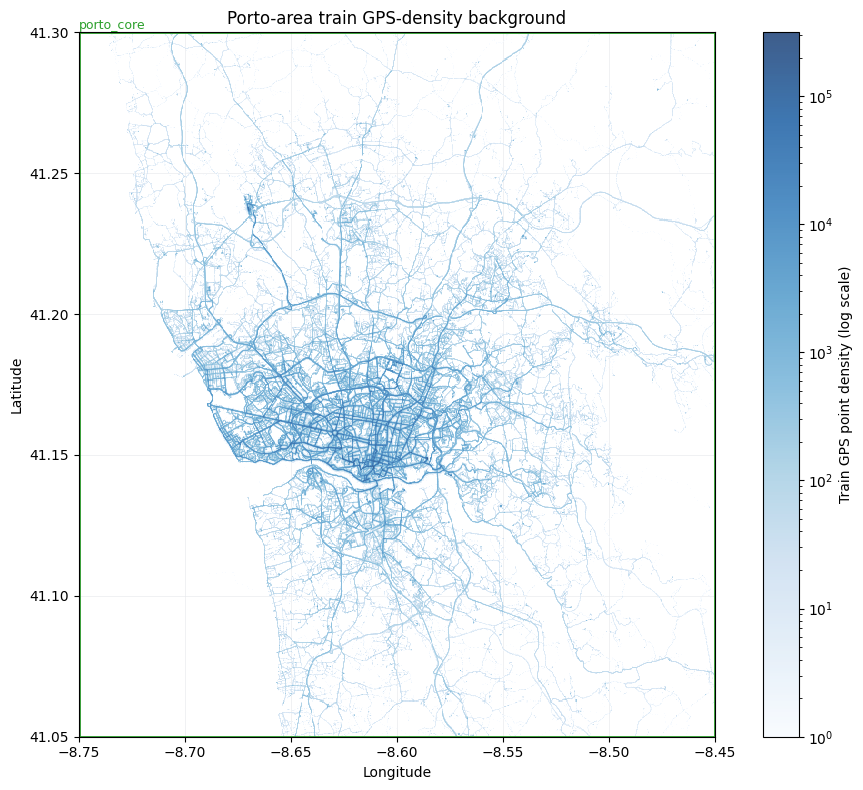
\includegraphics[width=0.52\textwidth]{../outputs/dataset_analysis/plots/porto_gps_density.png}
  \vfill
  {\large 17 July 2026\par}
  \vspace{0.7cm}
\end{titlepage}

\hypersetup{pageanchor=true}
\pagenumbering{roman}

\begin{abstract}
\setlength{\parskip}{0.55em}
We developed an end-to-end system for predicting the destination of a Porto taxi from a partially observed trajectory.  Starting from 1,710,670 labelled trips, we retained 1,672,901 after validity, spatial, and duration filtering.  We generated synthetic training prefixes with the same length distribution as the 320 supplied competition trajectories, then represented each prefix with its first and last GPS points, temporal variables, and dispatch metadata.  A shared 541-feature matrix supports six model families, while CatBoost uses a 36-column representation with native categorical variables.

We compared Linear Regression, Ridge, KNN, Decision Tree, Random Forest, XGBoost, and CatBoost under a common validation design, then combined the two strongest complementary models.  Random Forest achieved the best standalone results: 2.119~km on validation and 2.206~km on the 160-trip local public subset.  A fixed blend of 81.399\% Random Forest and 18.601\% XGBoost reduced the grouped cross-fitted validation error by 6.531~m on average and achieved the best local public score, 2.191~km.  The gain is consistent but small, so the main conclusion is that Random Forest provides the strongest individual model and XGBoost adds a modest corrective signal.  The principal limitations are the random rather than temporal validation split, repeated model selection on one holdout, and mixed CPU/GPU runtime measurements.

\end{abstract}
\clearpage

\begingroup
\small
\setstretch{1}
\setlength{\parskip}{0pt}
\setcounter{tocdepth}{2}
\tableofcontents
\listoffigures
\listoftables
\markboth{Contents and lists}{}
\endgroup
\clearpage

\pagenumbering{arabic}
\section{Introduction}

Destination prediction from a partial vehicle trajectory is a conditional forecasting problem: the observed path shows where a journey has been, but the unobserved suffix may still contain turns, detours, or a long final leg.  Accurate predictions can support taxi dispatch, demand anticipation, and passenger matching.  We study this problem with the Porto taxi data from the ECML/PKDD trajectory challenge \citep{moreira2015taxi}.  The task is to predict the final latitude and longitude of 320 trips from cut-off initial trajectories and trip metadata.

The competition metric is mean Haversine distance, so a useful model must control great-circle destination error rather than coordinate-wise error alone.  Our work addresses three questions:

\begin{enumerate}
  \item How should a variable-length partial trajectory be represented so that conventional regressors can predict a two-dimensional destination?
  \item Which linear, neighbourhood-based, single-tree, bagged-tree, and boosted-tree methods perform best under a shared validation protocol?
  \item Can a low-capacity blend improve the strongest standalone model without selecting its weight on the competition labels?
\end{enumerate}

Our final system has four main components:

\begin{itemize}
  \item one shared preprocessing pipeline for cleaning complete trajectories and constructing test-like partial prefixes;
  \item fixed-width spatial, temporal, and categorical features used consistently across model families;
  \item seven standalone regressors spanning simple baselines to GPU-accelerated boosting; and
  \item a grouped cross-fitted Random Forest--XGBoost blend selected before local competition scoring.
\end{itemize}

We use the validation holdout for model selection.  After the competition labels became locally available, we also score the frozen submissions on the 160-row public subset, the complementary 160-row private subset, and all 320 trips.  These local scores describe the final submissions; they are not used to learn the ensemble weight.  The public mean is the primary competition-facing result, while validation, tail error, and runtime provide complementary evidence.

\section{Data and feature construction}

\subsection{Task and data}

The training set contains \num{1710670} complete Porto taxi trajectories and the test set contains 320 partial trajectories.  Both CSV files use the nine-field schema in \cref{tab:dataset-schema}.  Each GPS point is recorded every 15 seconds as \texttt{[LONGITUDE, LATITUDE]}; the last point of a complete training polyline is the destination.  The test trips occur after the training year, so they introduce both a forecasting task and a temporal shift \citep{moreira2015taxi}.

\begin{table}[H]
  \centering
  \footnotesize
  \setlength{\tabcolsep}{4pt}
  \renewcommand{\arraystretch}{1.08}
  \begin{tabularx}{\linewidth}{@{}>{\ttfamily\raggedright\arraybackslash}p{2.5cm}>{\raggedright\arraybackslash}p{1.9cm}>{\raggedright\arraybackslash}p{2.8cm}X@{}}
\toprule
\multicolumn{1}{@{}l}{Field} & Type & Values / scope & Meaning \\
\midrule
TRIP\_ID & String & May repeat & Trip identifier. \\
CALL\_TYPE & Character & A, B, or C & Dispatch mode: central call, taxi stand, or street hail. \\
ORIGIN\_CALL & Integer & Type A; may be missing & Anonymized caller identifier when a central-call trip provides one. \\
ORIGIN\_STAND & Integer & Type B; otherwise missing & Taxi-stand identifier for stand-based trips. \\
TAXI\_ID & Integer & 442 taxis & Identifier of the taxi associated with the trip. \\
TIMESTAMP & Integer & Unix seconds & Trip start time. \\
DAY\_TYPE & Character & A, B, or C & Normal day, holiday, or day preceding a holiday, respectively. \\
MISSING\_DATA & Boolean & True or False & Whether the recorded GPS stream contains missing samples. \\
POLYLINE & List as string & Coordinate pairs & GPS samples stored as [LONGITUDE, LATITUDE] every 15 seconds; the final training point is the destination, whereas test rows contain only the observed prefix. \\
\bottomrule
\end{tabularx}

  \caption[Raw CSV schema]{Raw CSV schema.  Training and test files share these fields; in the test set, \texttt{POLYLINE} contains only the observed initial trajectory.}
  \label{tab:dataset-schema}
\end{table}

For an observed prefix
\begin{equation}
  P_i=\bigl((\lambda_{i1},\phi_{i1}),\ldots,
  (\lambda_{iL_i},\phi_{iL_i})\bigr),
\end{equation}
we predict the complete trip's final point $(\lambda_i^\star,\phi_i^\star)$.  Internally, every model uses the target order \texttt{[END\_LONG, END\_LAT]}; submission files convert this to \texttt{TRIP\_ID,LATITUDE,LONGITUDE}.  No external geographic data are used.

\begin{table}[H]
  \centering
  \small
  \begin{tabularx}{\linewidth}{@{}Xrr@{}}
\toprule
Population or representation & Rows & Features \\
\midrule
Raw training trajectories & 1,710,670 & 9 \\
Competition test prefixes & 320 & 9 \\
Retained training trajectories & 1,672,901 & 8 raw fields \\
Validation training matrix (default) & 1,338,320 & 541 \\
Validation holdout matrix (default) & 334,581 & 541 \\
Final training matrix (default) & 1,672,901 & 541 \\
Final training matrix (CatBoost) & 1,672,901 & 36 \\
\bottomrule
\end{tabularx}

  \caption[Populations and cached representations]{Populations and cached representations used in the experiments.}
  \label{tab:dataset-populations}
\end{table}

\begin{figure}[H]
  \centering
  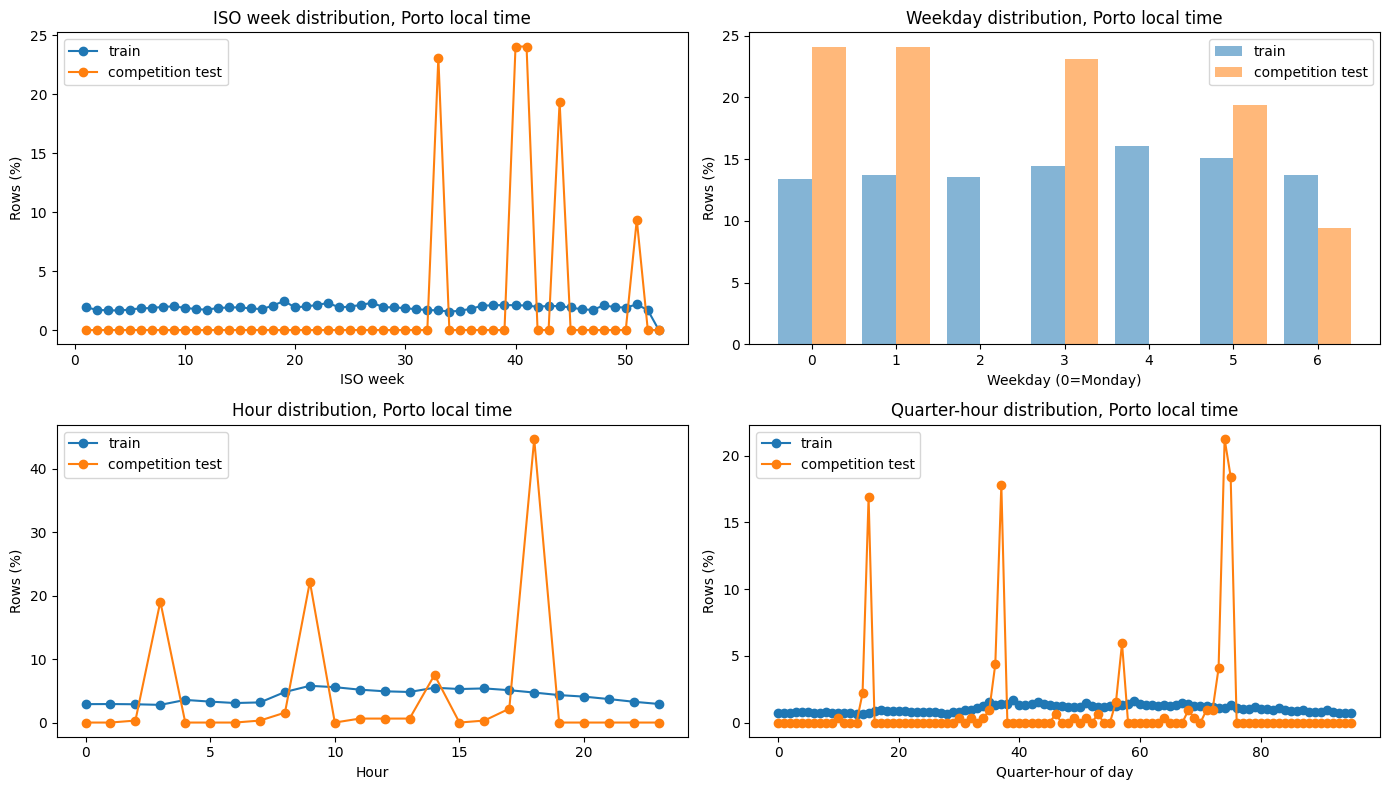
\includegraphics[width=\linewidth]{../outputs/dataset_analysis/plots/temporal_distributions.png}
  \caption[Temporal distributions of training trips and competition prefixes]{Temporal distributions of the training trips and the 320 competition prefixes in Porto local time.  The competition inputs are concentrated in later ISO weeks and a small set of observation times, motivating calendar features and caution when transferring results from a shuffled validation split.}
\end{figure}

\subsection{Cleaning and validation split}

We parse each polyline and remove incomplete, invalid, or shorter-than-two-point trajectories.  We then apply two conservative training-only checks: the first and final coordinates must fall inside a broad region around Porto, and GPS streams longer than four hours are removed only when they remain within 20~km of their start.  These steps remove 36,518 invalid or incomplete rows, 1,109 spatial outliers, and 142 duration artifacts, leaving \num{1672901} trajectories (97.792\% of the raw data).

Before feature construction, we create a shuffled 80/20 split with seed 42.  The resulting validation design contains \num{1338320} training rows and \num{334581} holdout rows.  Encoders, frequency statistics, and coordinate scaling are fitted on the training partition and then applied unchanged to the holdout.  For the final submissions, the same transformations are refitted on all retained trajectories.

\subsection{Competition-aligned synthetic prefixes}

The models must learn from complete training trajectories but predict from partial test trajectories of very different lengths.  We therefore generate one synthetic prefix per retained row in each partition:

\begin{enumerate}
  \item sample a desired length $L$ from the 320 supplied test-prefix lengths;
  \item select a training trajectory containing more than $L$ points;
  \item use its first $L$ points as input and its final point as target; and
  \item assert that the destination point is not present in the prefix.
\end{enumerate}

The supplied test trajectories were available during the competition, whereas their destinations and public/private membership were hidden.  Matching only their observable length distribution is therefore a competition-aligned use of the test inputs, not target leakage.  It produces synthetic prefixes with a median length of 26 points and a 95th percentile of 152 points, close to 26.5 and 152.15 in the test set.  A uniform cut-point strategy would instead produce much shorter examples, especially in the upper tail (\cref{fig:prefix-lengths}).  Seeds 42 and 43 generate the validation-training and validation-holdout prefixes; seed 142 generates a distinct full-data sample for final fitting.

\begin{figure}[H]
  \centering
  \begin{minipage}{0.88\linewidth}
    \centering
    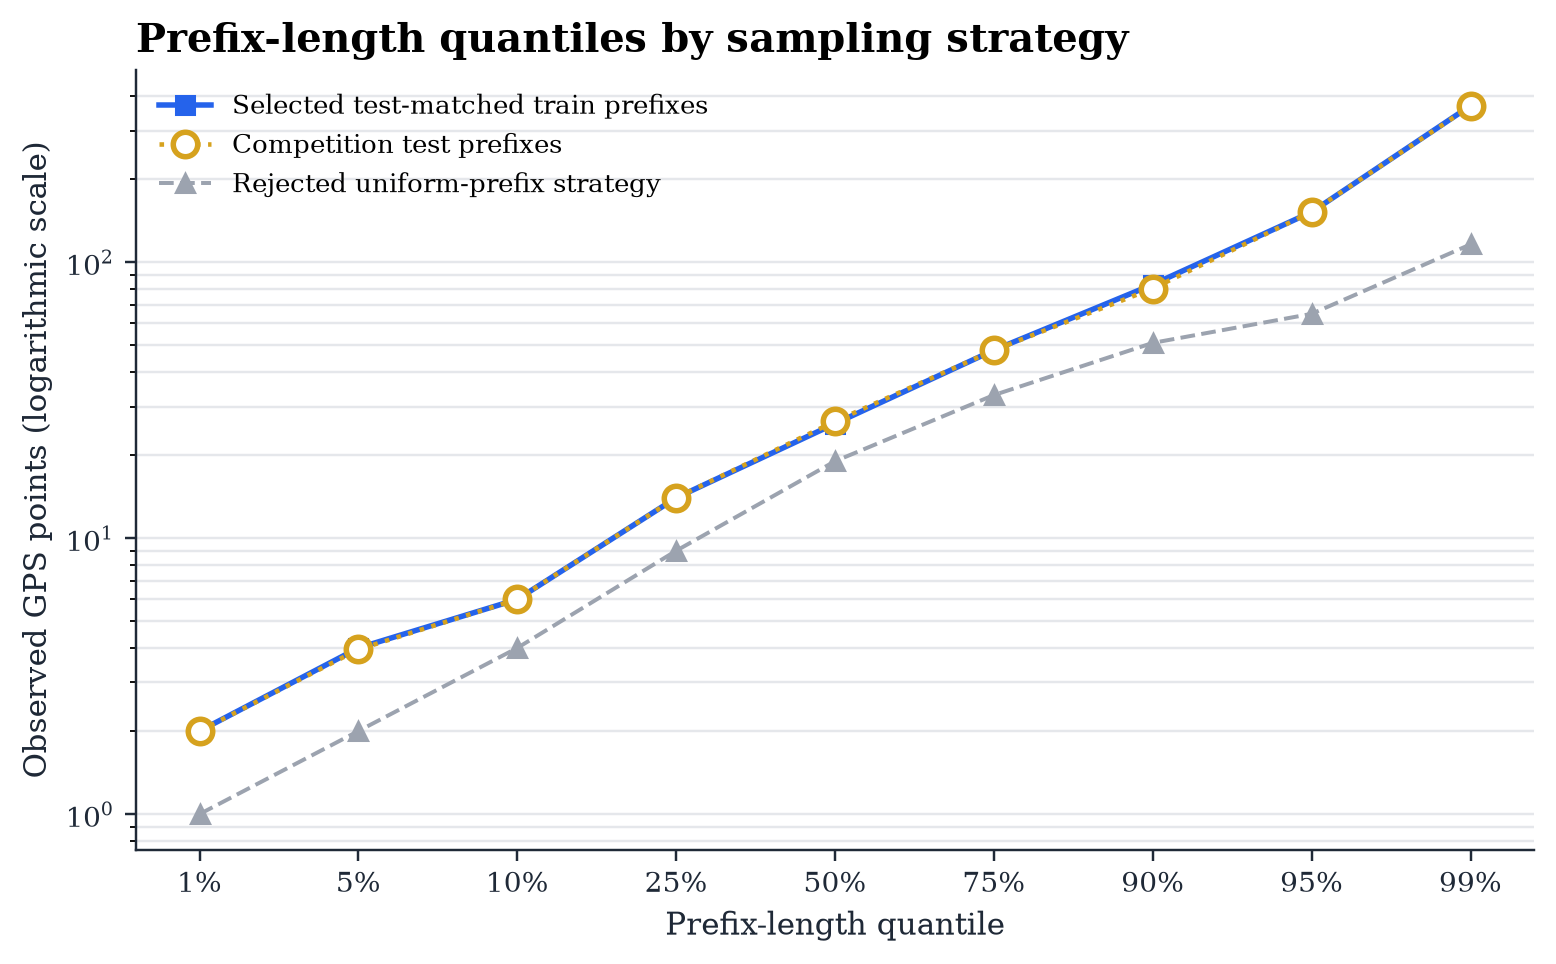
\includegraphics[width=\linewidth]{prefix_length_quantiles.png}
    \caption[Observed prefix-length quantiles]{Observed prefix-length quantiles.  The selected synthetic strategy follows the supplied test-prefix distribution much more closely than uniform cutting.  The vertical axis is logarithmic.}
    \label{fig:prefix-lengths}
  \end{minipage}
\end{figure}

\subsection{Fixed-width representation}

Each variable-length prefix becomes a fixed-width feature row.  We retain the first five and last five observed points in chronological order, giving 20 standardized coordinate features.  Short prefixes are padded with their edge coordinate.  We add 12 numerical features: caller missingness and log frequency, prefix length, local week, weekday, 15-minute quarter of day, and sine/cosine encodings of the three time cycles.

The default representation one-hot encodes \texttt{CALL\_TYPE}, \texttt{ORIGIN\_STAND}, and \texttt{TAXI\_ID}.  Its 541 columns decompose as
\begin{equation}
  20\ \text{GPS}+12\ \text{numeric}+3\ \text{call type}
  +64\ \text{stand}+442\ \text{taxi}=541.
\end{equation}
High-cardinality \texttt{ORIGIN\_CALL} is represented by missingness and log frequency rather than one-hot encoding.  CatBoost receives the same 32 numerical columns plus four native categorical variables---\texttt{CALL\_TYPE}, \texttt{ORIGIN\_CALL}, \texttt{ORIGIN\_STAND}, and \texttt{TAXI\_ID}---for 36 columns in total.  This gives all models the same spatial and temporal information while allowing CatBoost to use its native categorical treatment.

\section{Models}

We compare seven standalone regressors and one prediction-level ensemble.  Linear Regression, Ridge, KNN, Decision Tree, and Random Forest use scikit-learn \citep{pedregosa2011scikit}; XGBoost and CatBoost fit one regressor per coordinate.  Except for CatBoost's native categorical representation, every standalone model uses the same 541 input features.

\subsection{Linear and neighbourhood baselines}

\paragraph{Linear Regression and Ridge.}
Ordinary least squares provides a global additive baseline with an intercept and unconstrained coefficients.  Ridge Regression adds an $\ell_2$ penalty to stabilize the high-dimensional one-hot design \citep{hoerl1970ridge}; the selected value is $\alpha=316.23$.  Their similar results test whether the main limitation is coefficient variance or the absence of nonlinear spatial and categorical interactions.

\paragraph{K-nearest neighbours.}
KNN predicts a destination by averaging nearby training targets \citep{cover1967nearest}.  The accepted model uses brute-force Manhattan distance, $k=256$, and inverse-distance weighting on standardized features.  Because a full search is expensive at this scale, tuning and promotion use prefix-length-stratified samples; its validation value is therefore reported separately from the full-holdout evaluations.

\subsection{Tree-based models}

\paragraph{Decision Tree.}
The single-tree model supplies a nonlinear control \citep{breiman1984cart}.  Its selected configuration has depth 20, minimum split size 150, and minimum leaf size 20.  These node-size constraints regularize a tree that would otherwise memorize sparse taxi and stand indicators, but one axis-aligned partition remains sensitive to sampling variation.

\paragraph{Random Forest.}
Random Forest reduces that variance by averaging randomized trees \citep{breiman2001random}.  We select 700 bootstrap trees, depth 100, 50\% feature subsampling, and minimum split and leaf sizes of 5.  A slightly better validation mean was available, but the retained configuration reduced the 90th-percentile error by 2.447~m and trained about twice as fast in the recorded search.  This model becomes our strongest standalone system.

\paragraph{XGBoost.}
XGBoost fits a regularized sequence of trees to coordinate residuals \citep{chen2016xgboost}.  Longitude and latitude use depth-14 GPU models with learning rate 0.05, 90\% row subsampling, and 80\% column subsampling.  Early-stopped validation searches select different regularization and round counts for the two targets; full-data calibration then uses 625 rounds for longitude and 836 for latitude.

\paragraph{CatBoost.}
CatBoost combines boosting with native treatment of high-cardinality categorical variables \citep{prokhorenkova2018catboost}.  Its two GPU regressors use depth-10 symmetric trees, learning rate 0.03, $\ell_2$ leaf penalty 12, and Bayesian bootstrap.  Full-data calibration selects 3,207 iterations for longitude and 9,778 for latitude.  This model tests whether native caller, stand, and taxi identities improve on one-hot encoding.

\subsection{Random Forest--XGBoost ensemble}

Random Forest is the most accurate standalone model, while XGBoost offers a different residual pattern and a lower all-trip 90th-percentile error.  We combine their frozen coordinate predictions with one convex weight shared by longitude and latitude:
\begin{equation}
  \widehat{\boldsymbol y}(w)
  =w\widehat{\boldsymbol y}_{\mathrm{RF}}
  +(1-w)\widehat{\boldsymbol y}_{\mathrm{XGB}}.
  \label{eq:ensemble-blend}
\end{equation}
The final weight is
\begin{equation}
  \widehat{\boldsymbol y}
  =0.8139921906\,\widehat{\boldsymbol y}_{\mathrm{RF}}
  +0.1860078094\,\widehat{\boldsymbol y}_{\mathrm{XGB}}.
\end{equation}
Using one shared scalar keeps the ensemble deliberately low-capacity: XGBoost can correct part of the Random Forest error without introducing a coordinate-specific stacker that would be easier to overfit.

\section{Experimental design}

\subsection{Evaluation metric}

For a prediction $(\hat\lambda_i,\hat\phi_i)$ and destination $(\lambda_i,\phi_i)$, we compute the Haversine distance
\begin{align}
  a_i &= \sin^2\!\left(\frac{\phi_i-\hat\phi_i}{2}\right)
  +\cos(\hat\phi_i)\cos(\phi_i)
   \sin^2\!\left(\frac{\lambda_i-\hat\lambda_i}{2}\right),\\
  d_i &= 2R\,\operatorname{atan2}\!\left(\sqrt{a_i},\sqrt{1-a_i}\right),
  \qquad R=6371\ \mathrm{km},\\
  \mathcal L_{\mathrm{hav}}&=\frac{1}{n}\sum_{i=1}^{n}d_i.
\end{align}
Mean Haversine distance is the selection and competition metric.  Median and 90th-percentile distances are secondary diagnostics for the heavy error tail.  Most estimators optimize squared coordinate error internally, so all model decisions are made after recombining longitude and latitude and evaluating the geodesic metric.

\subsection{Model selection and final fitting}

All standalone models share the 80/20 synthetic-prefix holdout and the same feature definitions.  Linear Regression and Ridge use exhaustive finite grids; Decision Tree uses Optuna's tree-structured Parzen estimator \citep{akiba2019optuna}; Random Forest uses a reviewed finite grid; and KNN uses sampled search and promotion cohorts.  XGBoost and CatBoost use target-specific catalogues with early stopping, followed by a full-validation refit of the selected longitude/latitude pair.  Mean distance is primary, with tail error and runtime used to break practically negligible ties.

After selection, we rebuild the feature transformations on all \num{1672901} retained trajectories, calibrate the final boosting iteration counts where required, fit the accepted configuration, and predict the 320 test prefixes.  The final synthetic matrix uses prefix-sampling seed 142 to create a deterministic stream distinct from the validation samples; stochastic estimator seeds remain 42 where applicable.

\begin{figure}[H]
  \centering
  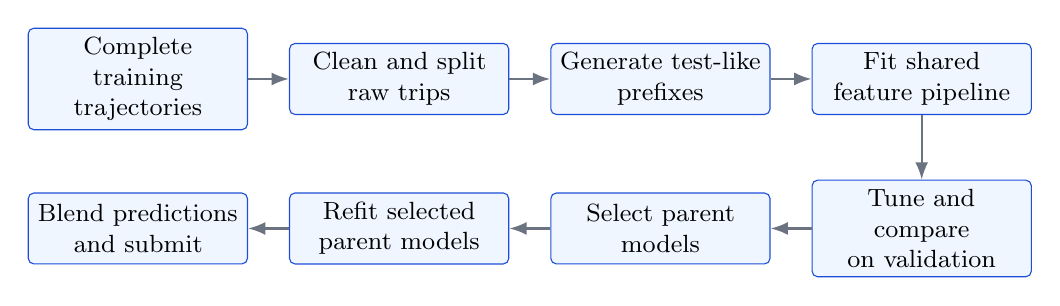
\begin{tikzpicture}[node distance=0.52cm and 0.52cm]
    \node[workflow] (raw) {Complete training\\trajectories};
    \node[workflow,right=of raw] (clean) {Clean and split\\raw trips};
    \node[workflow,right=of clean] (prefix) {Generate test-like\\prefixes};
    \node[workflow,right=of prefix] (features) {Fit shared\\feature pipeline};

    \node[workflow,below=0.82cm of features] (compare) {Tune and compare\\on validation};
    \node[workflow,left=of compare] (select) {Select parent\\models};
    \node[workflow,left=of select] (refit) {Refit selected\\parent models};
    \node[workflow,left=of refit] (submit) {Blend predictions\\and submit};

    \draw[flowarrow] (raw) -- (clean);
    \draw[flowarrow] (clean) -- (prefix);
    \draw[flowarrow] (prefix) -- (features);
    \draw[flowarrow] (features) -- (compare);
    \draw[flowarrow] (compare) -- (select);
    \draw[flowarrow] (select) -- (refit);
    \draw[flowarrow] (refit) -- (submit);
  \end{tikzpicture}
  \caption[Shared training, selection, and final-fitting workflow]{Shared training, selection, and final-fitting workflow.  The competition labels do not enter model selection or ensemble-weight estimation.}
\end{figure}

\subsection{Grouped ensemble selection}

The Random Forest and XGBoost validation predictions are aligned one-to-one with the same targets.  Synthetic sampling can draw the same source trajectory more than once, so we recover the source-trip group and use five repeats of five-fold \texttt{GroupKFold}.  In each fold, the weight in \cref{eq:ensemble-blend} is learned on four folds and evaluated on held-out trip groups.  This produces 25 out-of-fold comparisons with Random Forest.

We promote the blend only if at least four of five repeat means are positive and the trip-group robust 95\% interval for the mean gain is strictly above zero.  After this gate passes, we estimate one deployable weight from all \num{334581} aligned validation rows and apply it to the already-finalized parent submissions.  The local public and private labels are used only after the weight is frozen.

\subsection{Reported populations and reproducibility}

Validation results measure performance on synthetic prefixes drawn from the training year.  Local competition results use the released solutions: 160 rows marked public, 160 complementary private rows, and all 320 rows together.  We rank models by the local public mean because it matches the competition-facing comparison, while the validation estimate remains the basis for model selection.  Runtime values describe the recorded workflow rather than a hardware-normalized benchmark: linear and scikit-learn tree models ran on CPU, XGBoost and CatBoost on GPU, and KNN on sampled cohorts.

The workflow is reproducible from the shared builder \path{code/build_preprocessed_datasets.py}, the model notebooks, the cached preprocessing archives, and the selected-parameter artifacts.  Each notebook separates tuning, validation refit, and final fit so expensive stages can be rerun deliberately.  The report itself is regenerated without retraining by running \texttt{make} in \path{report/}; its asset script re-scores the saved submissions and rebuilds the figures and tables.

\section{Results}

\subsection{Random Forest is the strongest standalone model}

\Cref{tab:model-comparison} summarizes every final approach.  The Random Forest--XGBoost blend achieves the best local public mean, 2.191~km.  Random Forest follows at 2.206~km and is the best standalone model; XGBoost is third at 2.276~km.  The same three systems lead on the private and all-trip means.

\begin{table}[H]
  \centering
  \small
  \setlength{\tabcolsep}{5pt}
  \begin{tabular}{@{}rlrrrrr@{}}
\toprule
Rank & Model & Public & Private & All & Validation & Fit (s) \\
\midrule
1 & Ensemble$^{\dagger}$ & 2.191 & 2.500 & 2.346 & 2.113 & -- \\
2 & Random Forest & 2.206 & 2.514 & 2.360 & 2.119 & 25,546.1 \\
3 & XGBoost & 2.276 & 2.527 & 2.402 & 2.215 & 130.4 \\
4 & Decision Tree & 2.375 & 2.732 & 2.553 & 2.328 & 180.3 \\
5 & CatBoost & 2.390 & 2.565 & 2.478 & 2.297 & 473.0 \\
6 & Ridge & 2.665 & 3.107 & 2.886 & 2.888 & 28.1 \\
7 & Linear Regression & 2.668 & 3.099 & 2.883 & 2.891 & 53.1 \\
8 & KNN$^{\ddagger}$ & 3.351 & 3.568 & 3.460 & 3.566 & 0.577 \\
\bottomrule
\end{tabular}

  \vspace{0.35em}

  \begin{minipage}{0.96\linewidth}
    \footnotesize
    $^{\dagger}$The ensemble validation value is the mean of five repeated grouped cross-fits; the blend adds no new base-model fit.
    $^{\ddagger}$KNN validation and fit time use sampled promotion cohorts.  Other standalone validation values use the complete shared holdout.  Recorded fit times span CPU and GPU runs.
  \end{minipage}
  \caption[Final model comparison]{Final model comparison.  Distances are mean Haversine errors in kilometres; lower is better.  Public and private each contain 160 trips.}
  \label{tab:model-comparison}
\end{table}

The public ranking in \cref{fig:public-score-ranking} makes the top-level separation clear: the ensemble is first, Random Forest is the strongest standalone model, and XGBoost is the next-best complementary system.  The ensemble's 15.1~m advantage over Random Forest is nevertheless small relative to their roughly 2.2~km mean errors, so the chart should be read as a ranking rather than evidence of a large practical gap.

\begin{figure}[H]
  \centering
  \begin{minipage}{0.86\linewidth}
    \centering
    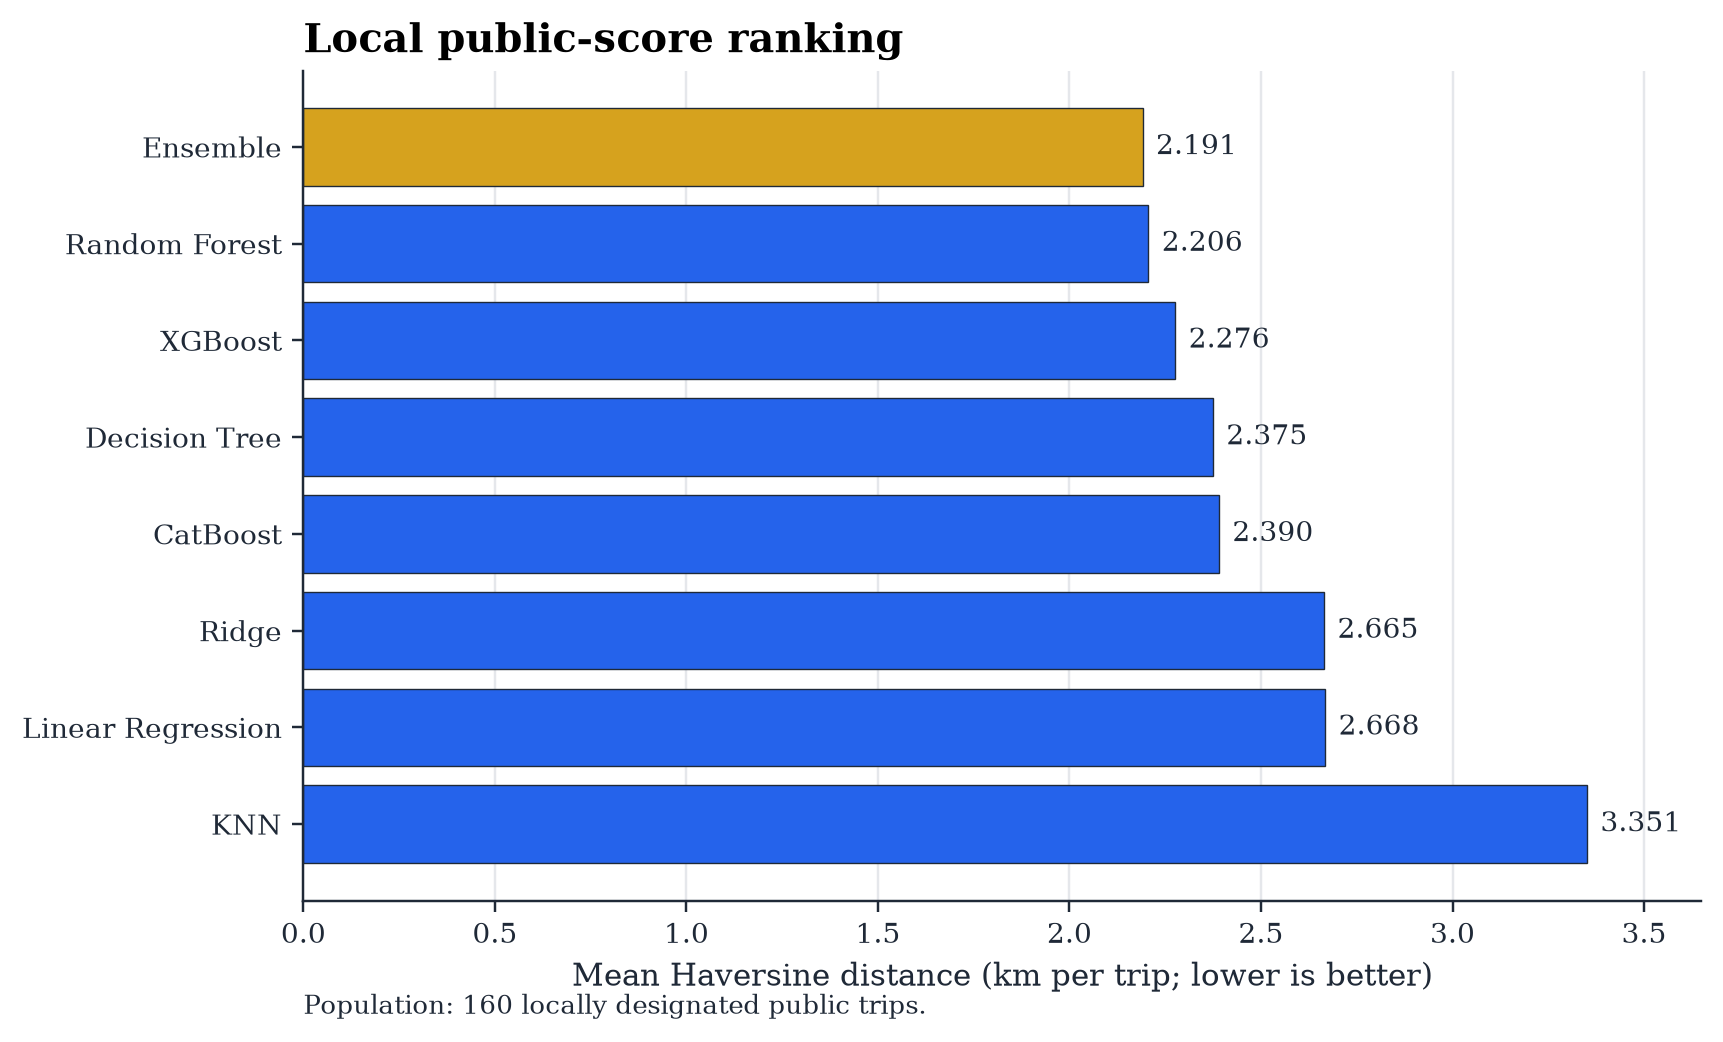
\includegraphics[width=\linewidth]{public_score_ranking.png}
    \caption[Local public-score ranking]{Local public-score ranking on the 160 trips designated public.  Bars show mean Haversine error in kilometres; lower is better, and gold highlights the promoted ensemble.}
    \label{fig:public-score-ranking}
  \end{minipage}
\end{figure}

The nonlinear tree families clearly outperform the linear and neighbourhood baselines.  Decision Tree improves the public mean by about 293~m relative to Linear Regression, and bagging reduces it by a further 168~m.  Ridge and Linear Regression are almost tied, showing that regularization does not overcome the missing nonlinear interactions.  KNN ranks last: Manhattan distance in a 541-dimensional mixed spatial and one-hot space is not an effective global notion of route similarity at this scale.

The lower ranks depend on the evaluated subset.  CatBoost is better than Decision Tree on validation, private mean, and all-trip mean, but Decision Tree is 15.8~m better on the public subset.  Ridge is 2.9~m better than Linear Regression publicly, while Linear Regression is slightly better on the private and all-trip means.  These small reversals should not be interpreted as stable superiority between close models.

\subsection{Validation and local scoring tell a consistent top-level story}

On the full standalone holdout, Random Forest scores 2.119~km, followed by XGBoost at 2.215~km, CatBoost at 2.297~km, Decision Tree at 2.328~km, Ridge at 2.888~km, and Linear Regression at 2.891~km.  KNN's 3.566~km value comes from its sampled promotion cohort and is not directly comparable.  The grouped cross-fitted ensemble reaches 2.113~km.  Thus validation and local competition scoring agree on the central conclusion: Random Forest is the strongest base model and XGBoost is the most useful complementary model.

Random Forest's advantage comes with substantial CPU cost.  Its accepted validation refit took 25,546~s, compared with 130~s for GPU XGBoost, 473~s for GPU CatBoost, and 180~s for Decision Tree.  XGBoost therefore provides the best observed accuracy--runtime compromise in this workflow.  The approximately $196\times$ Random Forest/XGBoost ratio is operational rather than algorithmic, because the runs use different hardware.

\subsection{The ensemble gain is consistent but small}

The frozen blend assigns 81.399\% weight to Random Forest and 18.601\% to XGBoost.  It improves on Random Forest in all 25 held-out group folds and in all five repeat means (\cref{fig:ensemble-repeat-gain}).  The mean cross-fitted gain is 6.531~m, with a trip-group robust 95\% interval of [4.555, 8.506]~m.  These results pass the pre-defined promotion gate and support using the blend instead of Random Forest alone.

\begin{figure}[H]
  \centering
  \begin{minipage}{0.84\linewidth}
    \centering
    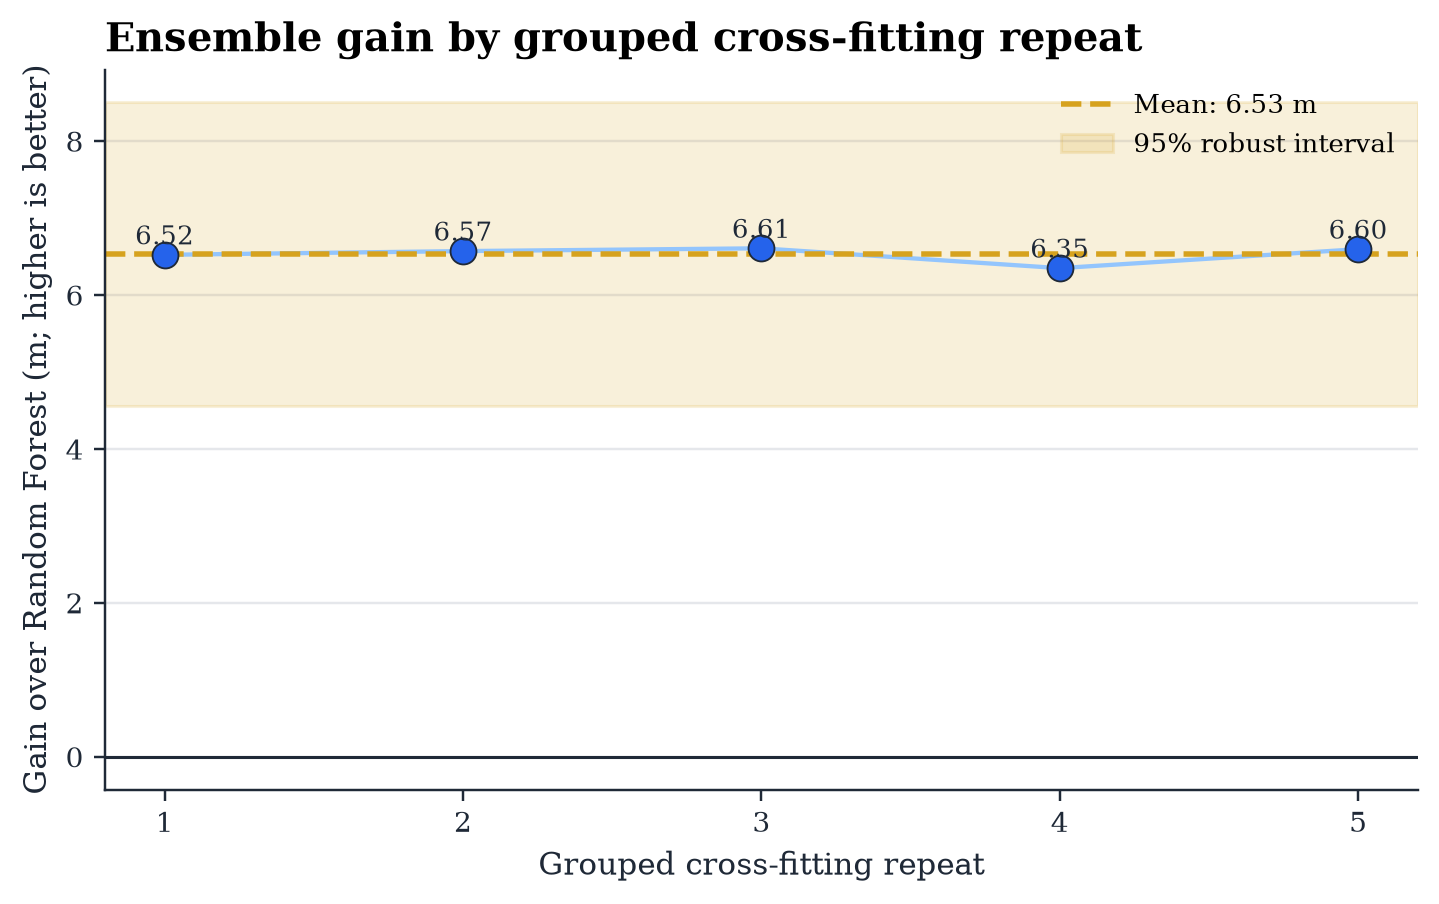
\includegraphics[width=\linewidth]{ensemble_repeat_gain.png}
    \caption[Mean ensemble gain over Random Forest by cross-fit repeat]{Mean ensemble gain over Random Forest in each repeated five-fold trip-group cross-fit.  Positive values favour the blend; the shaded band is the 95\% trip-group robust interval for the overall mean gain.}
    \label{fig:ensemble-repeat-gain}
  \end{minipage}
\end{figure}

On the local public subset, the ensemble improves the mean by 15.085~m (0.684\%) and ranks first at 2.191~km.  Across all 320 trips it improves the mean by 14.615~m.  The effect is not uniform: Random Forest has the slightly lower all-trip median (1.236 versus 1.257~km), while the ensemble has the lower 90th percentile (6.222 versus 6.243~km).  The blend is therefore an incremental correction that reduces some larger errors rather than a uniformly better prediction on every trip.

\section{Discussion, limitations, and next steps}

\subsection{Interpretation}

The main performance gap is between nonlinear tree models and the linear or distance-based baselines.  Recent coordinates, time, taxi identity, and dispatch context interact in ways that a global affine model cannot capture.  Random Forest benefits most from the large training population: deep randomized trees represent route-specific interactions, while averaging controls the instability of a single Decision Tree.  CatBoost's native categorical handling improves over the single tree on validation and all-trip mean, but it does not surpass Random Forest or XGBoost.  This suggests that spatial and temporal interactions matter more than native category processing alone.

The ensemble result is deliberately modest.  Random Forest supplies more than 81\% of the prediction, and XGBoost acts as a small corrective component.  Its gain is positive across every grouped fold, but 6.5~m is less than 0.4\% of the Random Forest validation error.  We therefore treat the blend as a justified final refinement, not as evidence that a more complicated stacking architecture is required.

The comparison also exposes a practical trade-off.  Random Forest is most accurate but expensive on CPU; XGBoost reaches a public error only 70~m higher with a much shorter GPU refit.  If training time or iteration speed matters, XGBoost is the more attractive standalone compromise.  The recorded timings should not be generalized beyond this hardware configuration.

\subsection{Limitations}

Our validation design is consistent across model families, but it is not a blind temporal test.  Training covers July 2013 to July 2014, whereas the competition trips occur later in 2014.  A shuffled holdout does not reproduce that shift, and duplicated trip identifiers or repeated synthetic source trips can weaken row-level independence.  Grouped folds address this issue for the ensemble-weight comparison, but the parent models were still selected on the common holdout.

Repeated tuning on one validation set introduces selection optimism, especially for the target-specific XGBoost and CatBoost searches.  The spatial and duration filters also use complete-trajectory information and therefore define performance only for the retained population.  These choices are reasonable for the competition pipeline, but the validation mean should not be interpreted as a fully unbiased estimate for future Porto trips.

Matching the synthetic prefix-length distribution to the 320 supplied test inputs is not leakage: no test destination or public/private label enters preprocessing.  It does, however, specialize the model to the competition's observed truncation pattern.  Performance under a different deployment policy, such as systematically shorter prefixes, would require a separate evaluation.

Finally, the released local solutions make it possible to compare all frozen submissions, but those labels should not be reused for further selection.  Public and private means contain only 160 trips each and can reverse close lower-model rankings.  We therefore base the ensemble decision on grouped validation and use local scores to describe the final competition outcome.

\subsection{Priorities for improvement}

Three extensions would strengthen the conclusions more than another broad search on the same holdout:

\begin{enumerate}
  \item \textbf{Grouped temporal validation.}  Train on earlier periods and reserve later trip groups for an outer assessment, with a separate inner split for feature, model, and ensemble selection.
  \item \textbf{Paired error analysis and nested blending.}  Retain source-row identifiers, evaluate errors by prefix length and trip context, and generate parent predictions inside each outer fold before learning the ensemble weight.
  \item \textbf{Standardized reproducibility and compute.}  Record one locked software environment and one hardware profile, then report training, prediction, model size, and memory use under comparable conditions.
\end{enumerate}

\section{Conclusion}

We built a common pipeline that converts complete taxi trajectories into competition-like partial prefixes, engineers a fixed spatial and contextual representation, and compares seven regression families.  Random Forest is the strongest standalone model, with mean Haversine errors of 2.119~km on validation and 2.206~km on the local public subset.  XGBoost is less accurate but substantially faster in the recorded GPU workflow and contributes complementary errors.

Our final 81.399\% Random Forest--18.601\% XGBoost blend achieves the best local public score, 2.191~km, and also ranks first on the private and all-trip means.  Its grouped cross-fitted gain averages 6.531~m and is positive in every fold, so the improvement is consistent but incremental.  The project therefore supports a simple conclusion: careful construction of test-like prefixes and a high-capacity Random Forest provide most of the performance, while a low-capacity blend offers a small final improvement.  A grouped temporal evaluation is the most important next step for measuring how well this result transfers beyond the competition split.


\clearpage
\phantomsection
\addcontentsline{toc}{section}{References}
\bibliographystyle{plainnat}
\bibliography{references}

\end{document}
